% 
% Annual Cognitive Science Conference
% Sample LaTeX Paper -- Proceedings Format
% 

% Original : Ashwin Ram (ashwin@cc.gatech.edu)       04/01/1994
% Modified : Johanna Moore (jmoore@cs.pitt.edu)      03/17/1995
% Modified : David Noelle (noelle@ucsd.edu)          03/15/1996
% Modified : Pat Langley (langley@cs.stanford.edu)   01/26/1997
% Latex2e corrections by Ramin Charles Nakisa        01/28/1997 
% Modified : Tina Eliassi-Rad (eliassi@cs.wisc.edu)  01/31/1998
% Modified : Trisha Yannuzzi (trisha@ircs.upenn.edu) 12/28/1999 (in process)
% Modified : Mary Ellen Foster (M.E.Foster@ed.ac.uk) 12/11/2000
% Modified : Ken Forbus                              01/23/2004
% Modified : Eli M. Silk (esilk@pitt.edu)            05/24/2005
% Modified: Niels Taatgen (taatgen@cmu.edu) 10/24/2006

%% Change ``a4paper'' in the following line to ``letterpaper'' if you are
%% producing a letter-format document.

\documentclass[10pt,letterpaper]{article}
\usepackage{url}
\usepackage{graphicx}
\usepackage{cogsci}
\usepackage{pslatex}
\usepackage{apacite}
\usepackage{amssymb,amsfonts,amsmath}
\usepackage{booktabs, colortbl, tabularx}
\usepackage[table]{xcolor}

\title{The Pragmatics of Metaphor Understanding: A Computational Approach}
 

  \author{{\large {\bf Justine T. Kao$^1$} (justinek@stanford.edu)}, {\large {\bf Leon Bergen$^2$} (bergen@mit.edu)}, {\large {\bf Noah D.~Goodman$^1$} (ngoodman@stanford.edu)}\\
  $^1$Department of Psychology, Stanford University. $^2$Department of Brain and Cognitive Science, MIT. }
 

\begin{document}

\maketitle
\begin{abstract}
Nonliteral language is, quite literally, everywhere, yet people's ability to use and understand it so effortlessly remains a mystery. Metaphor in particular has been studied extensively across many disciplines in cognitive science. One approach to studying metaphor focuses on the pragmatic principals that listeners utilize to infer meaning from metaphorical utterances. While this approach has generated fascinating theories and insights, to our knowledge there is no formal model showing that effects in metaphor understanding can arise from basic principles of communication. Building upon recent advances in formal models of pragmatics, we describe a computational model that interprets sentences metaphorically using pragmatic reasoning. We conduct behavioral experiments to evaluate the model's performance and show that our model produces metaphorical interpretations that closely fit behavioral data. We discuss implications of our model for metaphor understanding, principles of communication, and formal models of language understanding.

\textbf{Keywords:} 
language understanding; metaphor; pragmatics; computational models
\end{abstract}


\section{Introduction}
From ``Juliet is the sun" to ``No man is an island," nonliteral language is, quite literally, everywhere. Human communication is laden with metaphor and hyperbole, often creating poetic or humorous effects that add rich and important dimensions to language \cite{glucksberg2001understanding, pilkington2000poetic, lakoff2009more, roberts1994people, bergen2003cognitive}. Metaphor has inspired a particularly abundant amount of research in cognitive science, spanning topics such as how metaphors structure and shape our thoughts \cite{ortony1993metaphor, lakoff1993contemporary, thibodeau2011metaphors}, whether metaphor processing recruits the same strategies as standard language processing \cite{giora1997understanding, ortony1978interpreting, gibbs2002new, glucksberg1993metaphors} and what factors determine the meaning and aptness of a novel metaphor \cite{blasko1993effects, tourangeau1981aptness, kintsch2002metaphor}. The overwhelming interest in metaphor research is due in part to the ubiquity of metaphor in everyday language as well as the belief that metaphor may be critical for helping us understand how the mind creates meaning. 

One approach to studying metaphor focuses on the pragmatic principals that listeners utilize to infer meaning from metaphorical utterances \cite{tendahl2008complementary, stern2000metaphor}. Rather than view metaphor as a separate mode of communication that requires specialized language processing strategies, this approach argues that basic principles of communication drive the meaning that a listener infers from a metaphor \cite{sperber2008deflationary}. Relevance theory, in particular, posits that listeners interpret utterances with the assumption that speakers produced them because they are maximally relevant. Relevance theorists argue that this principle explains how listeners infer the meaning of a novel metaphor as well as other forms of loose talk where the meaning of the utterance is underspecified \cite{wilson2002relevance, wilson2006metaphor, sperber1985loose}. When interpreting the metaphor ``My lawyer is a shark," for example, the listener assumes that the speaker aims to communicate features of  ``a shark" that are relevant to the person under discussion (``my lawyer"), and thus do not make use of other shark features such as \emph{has fins} or \emph{swims}.

While many linguists and psychologists have argued for the benefits of studying metaphor using a pragmatics framework, to our knowledge there is no formal model showing that effects in metaphor understanding may arise from basic principles of communication. On the other hand, a recent body of work presents a series of computational models for pragmatic reasoning, where speaker and listener reason about each other to communicate effectively \cite{frank2012predicting, jager2009pragmatic}. By formalizing principals of communication, these Rational Speech Act models are able to quantitatively explain a range of phenomena in language understanding, such as scalar implicature and the effect of alternative utterances \cite{goodman2013knowledge, bergen2012s}. However, a limitation of these models is that they are unable to predict interpretations of an utterance that are false under its literal meaning. More recent work extends this model to consider affective goals in communication that may be optimally satisfied by nonliteral utterances such as hyperbole, which produced close quantitative fits with human interpretations (under review). In this paper, we consider communicative goals established by context that may be optimally satisfied by metaphorical utterances. In our formalization, a listener assumes that the speaker chooses an utterance to maximize informativeness about a subject along dimensions that are relevant to the conversation and consistent with the speaker's communicative goal. This makes it possible for a literally false utterance to be optimal as long as it is informative along the target dimension. Our framework closely aligns with the relevance-theoretic view that a listener considers the relevance of a meaning to the question under discussion in order to infer what the speaker intended to communicate. 

Although metaphor understanding is a complex phenomenon that calls for a variety of approaches, we present a computational model to argue that the interpretation of at least some types of metaphor are shaped at least in part by basic principals of pragmatics. To reasonably limit the scope of our work, we focus on metaphors of the classic form ``$X$ is a $Y$." We describe a computational model that can interpret such sentences metaphorically and conduct behavioral experiments to evaluate the model's performance. We show that peoples' interpretations of metaphors are driven by conversational context and that our model captures this effect. Finally, we show that our model predictions correlate significantly with people's fine-grained interpretations of metaphorical utterances.

\section{Computational Model}
At the core of basic Rational Speech Act models, a listener and a speaker recursively reason about each other to arrive at pragmatically enriched meanings. Given an intended meaning, a speaker reasons about a literal listener and chooses an utterance based on its informativeness. A pragmatic listener then reasons about the speaker and uses Bayes's Rule to infer the meaning given the utterance. To account for nonliteral interpretation, we extend this model by considering the idea that a speaker may have a range of different communicative goals. Intuitively, an utterance is optimally informative and relevant if it satisfies the speaker's communicative goal. Since the speaker's precise communicative goal may be unknown to the listener, the listener performs joint inference on the goal as well as the intended meaning. By introducing multiple potential goals for communication, we open up the possibility for a speaker to produce an utterance that is literally false but still satisfies her goal. The speaker achieves this in part by exploiting her own and the listener's prior knowledge---their common ground \cite{clark1996using}---to reason about what information the listener would gain if he takes the utterance literally. 

To illustrate this idea more concretely and demonstrate how it is implemented in our model, we will use the metaphor ``John is a shark" as an example. For simplicity, in this model we restrict the number of possible categories to which a member may belong to $c_a$ and $c_p$, denoting an animal category or a person category, respectively. We also restrict the possible features of John under consideration to a vector of size three: $\vec f = [f_1, f_2, f_3]$, where $f_i$ is either $0$ or $1$. We denote a possible communicative goal that a speaker may have as $g_{i,j}$, where $1 \leq i \leq 3$ and $j \in \{0,1\}$. $g_{i,j}$ is a function such that $g_{i,j} (\vec f) = 1$ if $f_i = j$, and $0$ otherwise, meaning a goal is satisfied if the listener correctly infers the value of a particular feature that the speaker cares to communicate about. 

Suppose the speaker $S_1$'s goal is to communicate that John has feature $f_1 =1$, where $f_1$ is the property \emph{scary}. $S_1$ reasons about a literal listener $L_0$ who will interpret an utterance ``John is a shark" as meaning that John is literally a member of the category ``shark." The literal listener is modeled as:
\[ L_0(c, \vec f |u) = \left\{ 
  \begin{array}{l l}
    P(\vec f | c) & \quad \text{if $c$ = $u$}\\
    0 & \quad \text{otherwise}
  \end{array} \right.\]

where $P(\vec f | c)$ is the prior probability that a member of a category $c$ (in this case ``shark" or 	``person") has feature values $\vec f$.

Given her goal, $S_1$ chooses an utterance $u$ according to a softmax decision rule that describes an approximately rational planner. $S_1$'s probability of producing utterance $u$ is therefore modeled as follows: \cite{sutton1998reinforcement}

\begin{equation}
S_1(u | g) \propto e^{\lambda U(u |  g)}
\end{equation}
where $U(u | g)$ describes the speaker's utility for producing $u$ given that she has goal $g$. Intuitively, $U(u |  g)$ can be quantified as the probability that the speaker's goal is satisfied subtracted by the cost of producing the utterance. Given an utterance $u$, the listener $L_0$ will guess that the meaning is $c, \vec f$ with probability $L_0 (c, \vec f|u)$. Since the goal function selects only certain meanings as relevant, the probability that the speaker's goal is satisfied by the utterance is $
\sum_{c, \vec f}{L_0 (c, \vec f|u) g(\vec f)}$. Optimizing the probability of the speaker's goal being satisfied can be accomplished by minimizing the goal's information-theoretic surprisal given an utterance. Using the information-theoretic definition of surprisal and a uniform utterance cost, equation (1) now becomes the following, where $\lambda$ is an optimality parameter:

\begin{equation}
S_1 (u | g) \propto \lambda \sum_{c,\vec f}{L_0 (c,\vec f|u) g(\vec f)}
\end{equation}

Intuitively, based on $S_1$'s understanding of $L_0$'s prior knowledge, she knows that if she produces the utterance ``John is a shark," $L_0$ will believe that John is literally a shark and hence very likely to be \emph{scary}. Since $S_1$'s goal is satisfied if the listener believes that John is scary, $S_1$ is motivated to produce such a metaphorical utterance. %the relationship between these quantities and surprisal might not be totally obvious -- it's probably worth at least noting that there are some computations not being shown here

A pragmatic listener $L_1$ now reasons about such a speaker. Based on prior knowledge, $L_1$ knows that John is extremely unlikely to be literally a member of the shark category. On the other hand, $L_1$ knows that the speaker $S_1$ is fairly likely to want to communicate about John's scariness. $L_1$ also knows that $S_1$ knows that \emph{scary} is a high-probability feature of sharks. The listener $L_1$ performs Bayesian inference to guess the intended meaning given prior knowledge and his internal model of the speaker. To determine the speaker's intended meaning, $L_1$ will marginalize over the possible speaker goals under consideration.
$$
L_1 (c, \vec f | u) \propto \sum_{g}{P(c) P(\vec f | c) P (g|\vec f) S_{1} (u|g)}
$$

Given $L_1$'s prior knowledge, his model of the speaker, and the utterance she produces, he infers that the meaning of the utterance is likely to be that John is a scary person. Note that while speaker and listener can continue to recursively reason about each other indefinitely, in this paper we present interpretation results for $L_1$.
\definecolor{Gray}{gray}{0.85}
\newcolumntype{a}{>{\columncolor{Gray}}c}
\begin{table*}[t]
\tabcolsep=0.05cm
\fontsize{8}{7.2}\selectfont
\begin{tabular}{a c c c c c c | a c c c c c c}
\toprule
Animal & $f_1=1$ & $f_2=1$ & $f_3=1$ & $f_1=0$ & $f_2=0$ & $f_3=0$ & Animal & $f_1=1$ & $f_2=1$ & $f_3=1$ & $f_1=0$ & $f_2=0$ & $f_3=0$ \\\hline
ant & small & strong & busy & large & weak & idle & goose & loud & mean & annoying & quiet & nice & agreeable \\
bat & scary & blind & nocturnal & unalarming & sighted & diurnal & horse & fast & strong & beautiful & slow & weak & ugly \\
bear & scary & big & fierce & unalarming & small & nonviolent & kangaroo & jumpy & bouncy & cute & relaxed & inelastic & unattractive \\
bee & busy & small & angry & idle & large & unangry & lion & ferocious & scary & strong & nonviolent & unalarming & weak \\
bird & free & graceful & small & unfree & awkward & large & monkey & funny & smart & playful & humorless & stupid & unplayful \\
buffalo & big & strong & wild & small & weak & tame & owl & wise & quiet & nocturnal & foolish & loud & diurnal \\
cat & independent & lazy & soft & dependent & fast & hard & ox & strong & big & slow & weak & small & fast \\
cow & fat & dumb & lazy & thin & smart & fast & penguin & cold & cute & funny & hot & unattractive & humorless \\
dog & loyal & friendly & happy & disloyal & unfriendly & unhappy & pig & dirty & fat & smelly & clean & thin & fragrant \\
dolphin & smart & friendly & playful & stupid & unfriendly & unplayful & rabbit & fast & furry & cute & slow & hairless & unattractive \\
duck & loud & cute & quacking & quiet & unattractive & non-quacking & shark & scary & dangerous & mean & unalarming & safe & nice \\
elephant & huge & smart & heavy & small & stupid & light & sheep & wooly & fluffy & dumb & hairless & hard & smart \\
fish & scaly & wet & smelly & smooth & dry & fragrant & tiger & striped & fierce & scary & unpatterned & nonviolent & unalarming \\
fox & sly & smart & pretty & artless & stupid & ugly & whale & large & graceful & majestic & small & awkward & inferior \\
frog & slimy & noisy & jumpy & nonslippery & quiet & relaxed & wolf & scary & mean & angry & unalarming & nice & unangry \\
goat & funny & hungry & loud & humorless & full & quiet & zebra & striped & exotic & fast & unpatterned & native & slow \\
\bottomrule

\end{tabular}
\caption{This table shows $32$ animal categories, feature adjectives, and their antonyms. Feature adjectives were elicited from Experiment 1a and indicate when a feature is present ($f_i = 1$). Antonyms were created using WordNet and indicate when a feature is not present ($f_i = 0$). Feature sets shown in Experiment 1b were created with this table, where $\vec f = [1, 0, 0]$ for category ``ant" is represented by the words $\{$small, weak, idle$\}$. There are $8$ possible feature combinations for each animal category.}
\end{table*}

To arrive at an interpretation, the listener needs to consider the following prior probabilities: 
\begin{itemize}
\item[(1)] $P(c)$, the prior probability that $X$ belongings to category $c$. We assume that $L_1$ is extremely certain that the person under discussion (e.g. John) is a person, but that there is a non-zero probability that John is actually a non-human animal. We fit $P(c_a)$ to data with the assumption that $10^{-4} \leq P(c_a) \leq 10^{-1}$.
\item[(2)] $P(\vec f | c)$, the prior probability that a member of category $c$ has feature values $\vec f$. We obtain this empirically in Experiment 1.
\item[(3)] $P(g | \vec f)$, the prior probability that given that a speaker knows the value of the feature vector $\vec f$, she wishes to communicate goal $g$. This prior can change given the the context that a question sets up. For example, if the speaker is responding to a vague question about John, e.g. ``What is John like?", the prior over goals is uniform. If the question is specific, such as ``Is John scary?", then she is much more likely to have the goal of communicating John's scariness. However, she may still want to communicate other features about John that were not asked about. We assume that the prior probability that $S_1$'s goal is to answer the specific question is greater than $0.5$ and fit the exact value to data.
\end{itemize}


\section{Behavioral Experiments}
To evaluate our model's interpretation of metaphorical utterances, we focused on a set of $32$ metaphors comparing human males to different non-human animals. We conducted Experiment 1a and 1b to elicit feature probabilities for the categories of interest. We then conducted Experiment 2 to measure people's interpretations of the set of metaphors. 

\subsection{Experiment 1a: Feature Elicitation}
\subsubsection{Materials}
We selected $32$ common non-human animal categories from an online resource for learning English (\url{www.englishclub.com}). The full list is shown in Table $1$.
\subsubsection{Methods}
$100$ native English speakers with IP addresses in the United States were recruited on Amazon's Mechanical Turk. Each subject read $32$ animal category names presented in random order, e.g. ``whale", ``ant", ``sheep". For each animal category, subjects were asked to type the first adjective that came to mind in a text box. 
\subsubsection{Results}
Using subjects' responses, we constructed a list of adjectives for each animal category and ordered them by the number of times they were given by a different subject (i.e. their popularity). We removed all color adjectives, such as ``brown" and ``black." To avoid constructing a set of features that have roughly equivalent meanings such as ``big", ``huge", and ``large", we used Wordnet \cite{Miller95wordnet:a} to identify synonymous adjectives and only kept the most popular adjective among a set of synonyms. We then took the top three most popular adjectives for each animal category and used them as the set of features. In what follows, $f_1$ is the most popular adjective, $f_2$ the second, and $f_3$ the third. Table 1 shows the animal categories and their respective features.

\subsection{Experiment 1b: Feature Prior Elicitation}
\subsubsection{Materials}
Using the features collected from Experiment 1a, we elicit the prior probability of a feature vector given an animal or person category (i.e. $P(\vec f | c)$). We assume that the adjective corresponding to a feature (e.g. \emph{scary}) indicates that the value of that feature is $1$ (present), while the adjective's antonym indicates that the value of that feature is $0$ (not present). We used Wordnet to construct antonyms for each of the adjective features produced in Experiment 1a. When multiple antonyms existed or when no antonym could be found on Wordnet, the first author used her judgment to choose the appropriate antonym. Table 1 shows the resulting list of antonyms. 

For each animal category, eight possible feature combinations were constructed from the three features and their antonyms. For example, the possible feature combinations for a member of the category ``ant" are \{small, strong, busy\}, \{small, strong, idle\}, \{small, weak, busy\}, and so on.

\subsubsection{Methods}
$60$ native English speakers with IP addresses in the United States were recruited on Amazon's Mechanical Turk. Each subject completed $16$ trials in random order. Each trial consisted of the eight feature combinations for a particular animal category. Using slider bars with ends marked by ``Impossible" and ``Absolutely certain," subjects were asked to rate how likely it is for a member of the animal category to have each of the eight feature combinations. Subjects also rated the probabilities of the feature combinations for a male person. We only elicited priors for males in order to be consistent with Experiment 2 and minimize confounds with gender.

\subsubsection{Results} 
We normalized each subject's ratings for the eight feature combinations in a trial to sum up to 1 based on the assumption that the eight feature combinations exhaustively describe a member of a particular category. Averaging across subjects' normalized ratings, we obtained the feature priors $P(\vec f | c)$ for $c = c_a$ (animal) and $c = c_p$ (person).
%, where $f_i = 1$ is represented by the feature adjective and $f_i = 0$ is represented by its antonym. 
Figure~\ref{prior} shows the average marginal probabilities of features being present given an animal category and a person category. Since the features were created using the animal categories in Experiment 1a, by construction features are rated as significantly more likely to be present in the animal category than in the person category ($F(1, 190) = 207.1$, $p < 0.0001$). These results confirm that subjects are fairly confident that each animal category has certain distinguishing features (mean$= 0.61$, sd$=0.06$), while those same features are rated as appearing in people with roughly $0.5$ probability (mean$=0.48$, sd$=0.06$).
\begin{figure}[t]
\begin{center}
\scalebox{0.6}{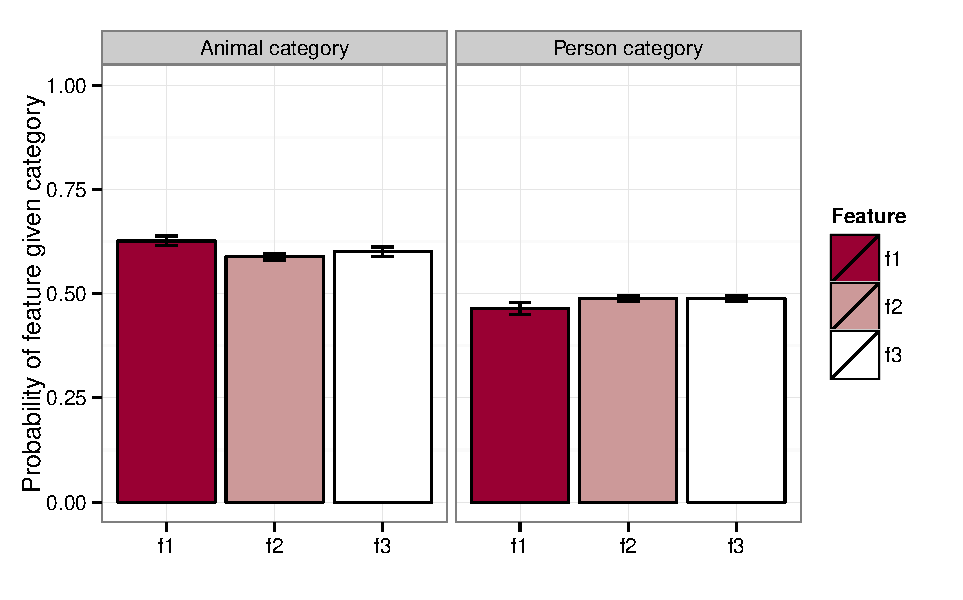
\includegraphics{Plots/priors_bar.pdf}}
\end{center}
\caption{Average marginal prior probability ratings for the three features given an animal category or a person category. Error bars are standard error over the $32$ items.} 
\label{prior}
\end{figure}

\subsection{Experiment 2: Metaphor Understanding}
\subsubsection{Materials}
We created $32$ scenarios based on the animal categories and results from Experiment 1. In each scenario, a person (e.g. Bob) is having a conversation with his friend about a person that he recently met. Since we are interested in how the communicative goals set up by context affect metaphor interpretation as well as the effectiveness of metaphorical versus literal utterances, we created four conditions for each scenario by crossing vague/specific goals and literal/metaphorical utterances. In vague goal conditions, Bob's friend asks a vague question about the person Bob recently met: ``What is he like?" In specific goal conditions, Bob's friend asks a specific question about the person: ``Is he $f_1$?" Where $f_1$ is the most popular adjective for a given animal category $c_a$. In literal conditions, Bob replies with a literal utterance, either by saying ``He is $f_1$." to the question ``What is he like?" or ``Yes." to the question ``Is he $f_1$?". In Metaphorical conditions, Bob replies with a metaphorical statement, e.g. ``He is a $c_a$." where $c_a$ is an animal category. See Table 2 for examples of each condition.

\begin{figure}[t]
\begin{center}
\scalebox{0.6}{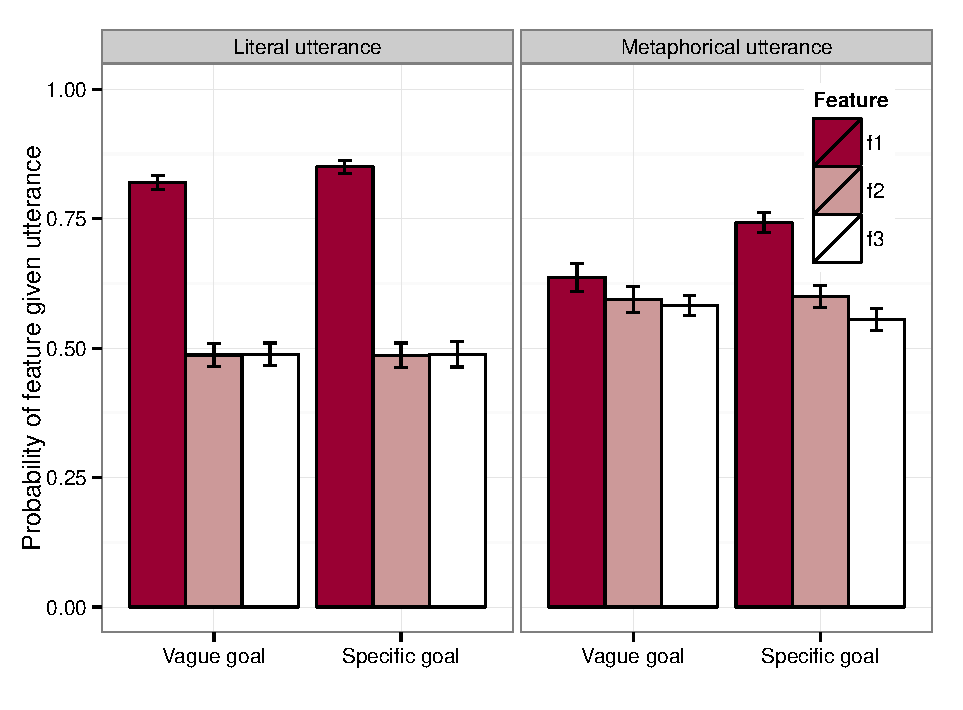
\includegraphics{Plots/human_bar.pdf}}
\end{center}
\caption{Average probability ratings for the three features given a vague/specific goal and a literal/metaphorical utterance. Error bars are standard error over the $32$ items.} 
\label{human_bar}
\end{figure}

\subsubsection{Methods}
$49$ native English speakers with IP addresses in the United States were recruited on Amazon's Mechanical Turk. Each subject completed $32$ trials in random order. The $32$ trials were randomly and evenly assigned to one of the four conditions, i.e. each subject read $8$ scenarios for each condition. For each trial, subjects used sliders to indicate the probabilities that the person described has features $f_1$, $f_2$, and $f_3$, respectively.

\begin{table}
\tabcolsep=0.2cm
\small
\begin{tabular}{llll}
\toprule
Goal & Utterance & Example question & Example utterance \\
\midrule
Vague & Literal & ``What is he like?" & ``He is scary." \\
Specific  & Literal & ``Is he scary?" & ``Yes." \\
Vague & Metaphorical & ``What is he like?" & ``He is a shark." \\
Specific & Metaphorical & ``Is he scary?" & ``He is a shark." \\
\bottomrule
\end{tabular}
\caption{Example scenarios given the four experimental conditions in Experiment 2.s}
\end{table}

\subsubsection{Results}
\begin{figure}[ht]
\begin{center}
\scalebox{0.6}{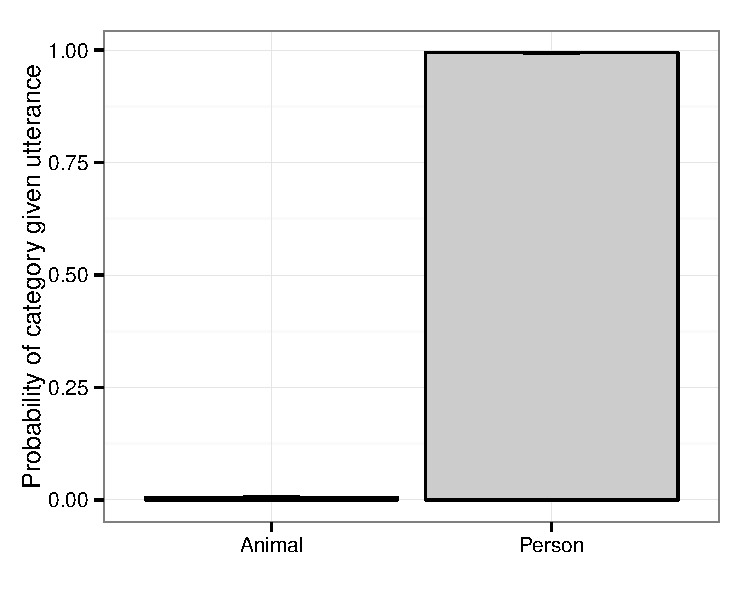
\includegraphics{Plots/model_literal.pdf}}
\end{center}
\caption{Model's average marginal category probabilities given a metaphorical utterance ($P(c | u)$). Model's prediction for the animal category is close to $0$ and close to $1$ for the person category. Error bars are standard error over the $32$ items.} 
\label{scatter_full}
\end{figure}
For each condition of each scenario, we obtained the average probability ratings for the three features. Figure~\ref{human_bar} shows the average ratings for each feature across animal categories given a vague or specific goal and a literal or metaphorical utterance. We see that when the speaker gives a literal statement directly affirming the presence of $f_1$, subjects rate $f_1$ as significantly more likely than when the speaker gives a metaphorical statement ($F(1, 126) = 52.6$, $p < 0.00001$). However, subjects rate $f_2$ and $f_3$ as significantly more likely when the speaker produces a metaphorical utterance ($F(1, 126) = 23.7$, $p < 0.0001$; $F(1, 126) =13.66$, $p < 0.0005$). We also see an effect of the speaker's communicative goal on the interpretation of metaphorical utterances. Given a specific question about $f_1$, subjects interpret the speaker's metaphorical utterance as being relevant to the question and rates the probability of $f_1$ as significantly higher than when the question is vague ($F(1, 62) = 10.16$, $p < 0.005$). On the other hand, the probabilities of $f_2$ and $f_3$ are not significantly different given a vague question or a specific question about $f_1$ ($F(1, 62) = 0.03788$, $p > 0.05$; $F(1, 62) = 0.8285$, $p > 0.05$). When comparing to the feature priors for the person category in Figure $1$, we see that given a metaphorical utterance, subjects are much more likely to infer that the person described has features of the animal in the metaphor.

\section{Model Evaluation}
We used the feature priors obtained in Experiment 1b to compute model interpretations of the $32$ metaphors. The behavioral results in Experiment 2 show evidence that the context set up by a question changes subjects' interpretation of a metaphor. Our model naturally accounts for this using the speaker's prior over communicative goals $P(g | \vec f)$ under different conversational contexts. When a speaker is responding to a vague question, we set the prior distribution for $P(g | \vec f)$ as uniform. When the speaker is responding to a question specifically about $f_1$, we assume that the $P(g_1 | \vec f) > 0.5$ and equal among $P(g_2 | \vec f) = P(g_3 | \vec f)$. Fitting the goal prior parameter to data yields a prior of $P(g_1 | \vec f) = 0.6$ when responding to a specific question about $f_1$. We fit the category prior $P(c_a) = 0.01$ and the speaker optimality parameter $\lambda = 3$.

Using these parameters and the model we described, we obtained interpretation probabilities for each of the $32$ metaphors under both vague and specific goal conditions. For each metaphor and goal condition, the model produces a joint posterior distribution, $P(c, \vec f | u)$. We first show a basic but important qualitative result, which is that the model is able to interpret utterances metaphorically. The pragmatic listener successfully infers that the person described is actually a person and not an animal. Marginal over values of $\vec f$, the probability of the person category is close to one ($P(c_p | u) = 0.994$), indicating that the model is able to combine prior knowledge and reason about the speaker's communicative goal to arrive at nonliteral interpretations (Figure 3).

%\begin{figure}[t]
%\begin{center}
%\scalebox{0.6}{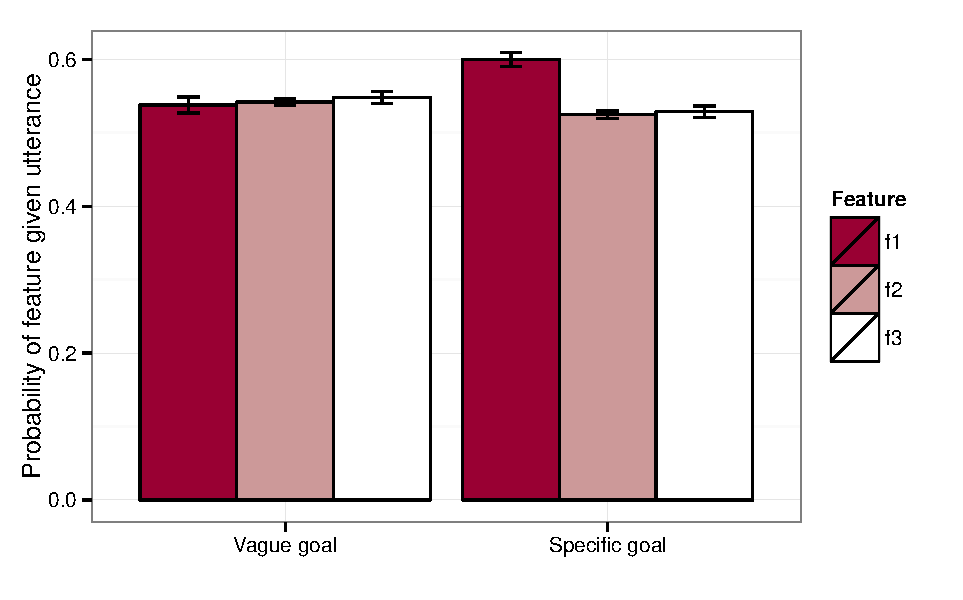
\includegraphics{Plots/model_bar.pdf}}
%\end{center}
%\caption{Model's average } 
%\label{scatter_full}
%\end{figure}

\begin{figure}[t]
\begin{center}
\scalebox{0.6}{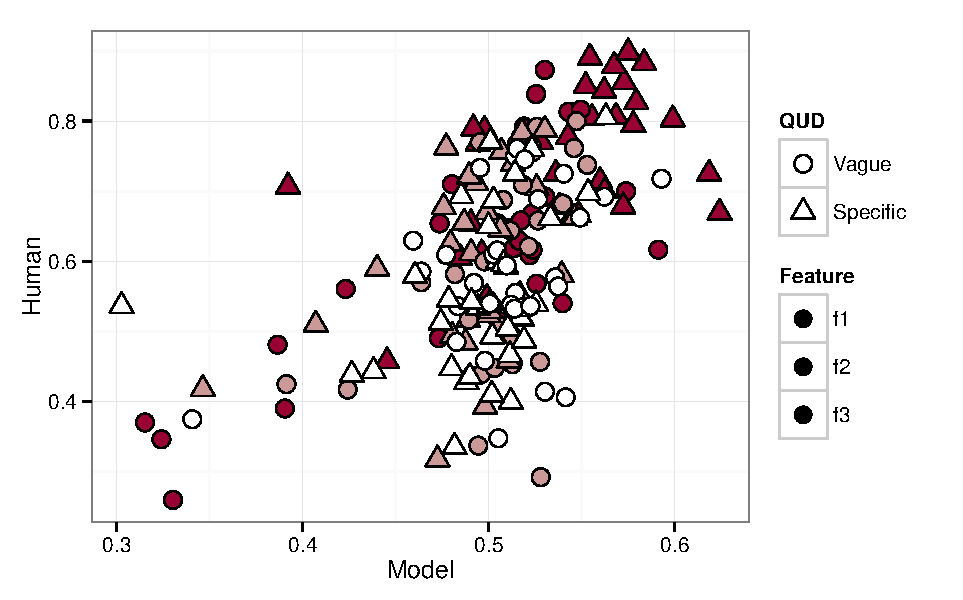
\includegraphics{Plots/scatter_full.pdf}}
\end{center}
\caption{Model predictions ($x$ axis) vs subjects' probability ratings ($y$ axis) for $192$ items ($32$ metaphors $\times$ $3$ features $\times$ $2$ goal conditions). Shape of points indicates goal condition and color indicates feature number.} 
\label{scatter_full}
\end{figure}

We now turn to the second component of the interpretation, $P(\vec f | u)$. 
%Figure X shows the average marginal feature probabilities given a vague or specific goal. The model's interpretations are shaped by the communicative goal set up by context, where $f_1$ receives significantly higher marginal probabilities when the speaker is responding to a specific question about $f_1$ ($F(1, 62) =17.92$, $p<0.0001$). This qualitatively matches behavioral results in Figure X. 
To quantitatively evaluate the model's performance, we correlated model predictions with human interpretations of the metaphorical utterances. Given a metaphorical utterance and a vague or specific question condition, we computed the model's marginal posterior probabilities for $f_1$, $f_2$, and $f_3$. We then correlate these posterior probabilities with subjects' probability ratings from Experiment 2. Figure 4 plots model interpretations for all metaphors, features, and goal conditions against human judgments. Correlation across the $192$ items ($32$ metaphors $\times$ $3$ features $\times$ $2$ goal conditions) is $0.6$ ($p < 0.001$). The predicted reliability of subjects' ratings using the Spearman-Brown prediction formula is $0.83$, suggesting first that people do not always agree on metaphorical interpretations, and second that our model captures a significant amount of the reliable variance in the behavioral data. In particular, our model does especially well at predicting subject's judgments of $f_1$, which are the most salient features of the animal categories and were targeted by specific questions in Experiment 2. Correlation between model predictions and human judgments for $f_1$ is $0.7$ ($p < 0.0001$), which is close to the predicted reliability of subjects' ratings for $f_1$, $r=0.82$. 

We now compare our model's performance to a reasonable baseline model that considers the feature priors for animals and people as well as the conversational context. We constructed a linear regression model that takes the marginal feature priors for the animal category, the marginal feature priors for the person category, and the vague or specific goal as predictors of subjects' ratings. This model produced an adjusted $R^2 = 0.19$ ($r = 0.44$), which is a significantly worse fit than our model ($p < 0.0001$ on a Cox test). This suggests that our computational model adequately combines people's prior knowledge about the source and target domains as well as principals of pragmatics to produce metaphorical interpretations that closely fit behavioral data.

While our model captures a significant amount of reliable variance, here we perform in-depth analysis of the metaphors and features for which our model performs less well.

\section{Discussion}
In this paper we presented a computational model that predicts rich metaphorical interpretations by formalizing principals of communication. Besides going beyond the literal meaning of an utterance to infer non-literal interpretations (i.e. John is a person and not a shark), our model is able to quantitatively predict fine-grained judgments about the person's features (i.e. John is very likely scary, dangerous, and mean). Furthermore, behavioral results show that the interpretation of a metaphor is shaped in part by the conversational context, which our model naturally accounts for by adjusting the priors over conversational goals. Together these results suggest that basic principals of communication may be an important driver of metaphor understanding.

Our model captures several important intuitions about communication, including the importance of common ground between listener and speaker, the communicative goals shaped by the conversational context, and the idea that speakers choose to produce utterances that maximize informativeness about features relevant to their communicative goal. Each of these components inspire research questions that can be further investigated using both our modeling framework and experimental paradigm. For example, are listeners less likely to interpret an utterance metaphorically when there is little common ground between speaker and listener? Does speaking metaphorically allow speakers to respond to specific questions while simultaneously introducing new information that they may wish to communicate? We aim to address these questions in future research to further clarify how components of communication interact to produce metaphorical meaning. We believe that our computational framework for modeling language understanding advances our knowledge of the computational basis of metaphor and other types of nonliteral language, and we hope that it will continue to shed metaphorical light on related questions.

\section{Acknowledgments}

Place acknowledgments (including funding information) in a section at the end of the paper.



\bibliographystyle{apacite}

\setlength{\bibleftmargin}{.125in}
\setlength{\bibindent}{-\bibleftmargin}

\bibliography{metaphor}


\end{document}
